\documentclass[twoside]{article}
\usepackage{mathpazo}
\usepackage[T1]{fontenc}
\usepackage[utf8]{inputenc}
\usepackage{graphicx}
\usepackage[colorlinks]{hyperref}
\hypersetup{
  colorlinks,
  urlcolor=blue,
  linkcolor=black
}
\usepackage{caption} % unnumbered video examples
% \usepackage{authblk} % author affiliations
\usepackage{hanging} % hanging indents

% headers
\usepackage{fancyhdr}
\renewcommand{\headrulewidth}{0pt}

% first page footer
\fancypagestyle{infofooter}{%
  \fancyhf{}
  \renewcommand\headrulewidth{0pt}
  \fancyfoot[L]{\sffamily\small 
    WORLD MUSIC TEXTBOOK, ISSN: 2767-4215; \copyright~2020, CC-ND-BY-ND\\
    http://dx.doi.org/XX.XXXX/XXXXXXXX.2021.XXXXXXX}
}
\thispagestyle{infofooter} % remove header from first page
\pagestyle{fancy}     % add headers in other pages

% normal headers
\fancyhead[LO]{\sffamily\small \textbf{\thepage} \quad World Music Textbook}
\fancyhead[RE]{\sffamily\small McNally: Articulating Race and Nation in Brazilian Popular Song \quad \textbf{\thepage}}
\fancyfoot{}

% flush left title
\makeatletter
\renewcommand{\maketitle}{\bgroup\setlength{\parindent}{0pt}
\begin{flushleft}
  \vspace*{3\baselineskip}
  \huge{\textbf{\@title}}

  \medskip
  
  \large{\@author}
\end{flushleft}\egroup
}
\makeatother

% for keywords and abstract
\providecommand{\abstracttext}[1]
{
  \noindent
  \textbf{Abstract:} #1
}

\providecommand{\keywords}[1]
{
  \newline
  \textbf{Keywords:} #1
}

% for link
\providecommand{\wmturl}{\href{https://worldmusictextbook.org/mcnally-2021}{https://worldmusictextbook.org/mcnally-2021}}
\providecommand{\wmturltext}{
  \noindent\emph{The online version of this chapter includes all embedded content and is available at \wmturl.}
}
\providecommand{\wmturlcaption}{
  Visit \href{https://worldmusictextbook.org/mcnally-2021}{the website} to view video examples.
}

% metadata
\title{Articulating Race and Nation in Brazilian Popular Song}
\author{James McNally | University of Illinois at Chicago}
% \affil{}

\date{}

% document
\begin{document}
\suppressfloats % prevent float above title
\maketitle

\abstracttext{This article presents a cultural history of Brazilian popular song (canção popular) and the many musical genres that fall under its umbrella. From the early days of samba to contemporary popular styles, popular song in Brazil has long represented a site for negotiating complex questions of race, nation, and politics.}
\keywords{activism, nationalism, politics, popular music, race, Latin America, South America}

\smallskip

\wmturltext

\medskip

\noindent\hfil\rule{0.5\textwidth}{0.4pt}\hfil

\bigskip

\section*{Part 1}

Since the beginning of the twentieth century, the dominant musical form
in the Brazilian cultural sphere has been popular song, or \emph{canção
popular} (often shortened to \emph{canção}, or ``song''). The term
encompasses a range of song-based musical genres, from the poignant
midcentury ballads of \emph{samba-canção} to widely circulating
contemporary styles such as \emph{sertanejo}.\footnote{For a discussion
  of the nuances of the Portuguese language term \emph{canção} and how
  it differs from the more general English language term ``song,'' see
  McNally 2021, 128.} Studies of Brazilian popular song typically focus
on the work of individual singer-songwriters, or \emph{cancionistas}, on
whom literature on the subject is predominantly concentrated.\footnote{See,
  e.g., Napolitano 2001; Tatit 1996; 2002; 2004. The term
  \emph{cancionista} was most prominently introduced and pioneered by
  Luiz Tatit.} In addition to shaping the invention of new song-based
genres over time, these figures also acted as cultural commentators
throughout periods of social and political crisis, whether in opposition
to the 1964-85 military dictatorship or speaking out against racial
inequality. Through their recordings, they also acted as ambassadors for
creating notions of a common Brazilian musical language as well as a
sense of unity across the country's diverse panorama of cultures and
communities, from the interior towns of the arid Northeastern
\emph{sertão} to the hillside neighborhoods of Rio de Janeiro. As this
chapter will show, even as popular song has maintained certain core
structural qualities, it has long acted as a site for political
contestation, social commentary, creative transformation, and the
construction of national identity. To examine popular song and its
various constituent genres is to gain a window into Brazilian cultural
politics over time and the creative strategies musicians have employed
to participate in these societal shifts.

\hypertarget{the-early-years}{%
\subsection*{The Early Years}\label{the-early-years}}

Brazilian popular song first appeared in national media in the late
1910s and 1920s with the introduction of early recording technology.
Samba, along with related genres such as \emph{maxixe}, constituted an
early stylistic template for the form.\footnote{Early samba drew heavily
  from creolized urban dance genres circulating in late-nineteenth and
  early-twentieth century Rio de Janeiro such as \emph{maxixe},
  \emph{tango brasileiro,} and the instrumental genre of \emph{choro,}
  all of which mixed Afro-Brazilian practices with genres circulating in
  the broader international sphere, both within and beyond Latin
  America.} Scholar and songwriter Luiz Tatit identifies the ``encounter
between \emph{sambistas} and the gramophone'' in the late 1910s as a
starting point for ``what we know today as popular song'' (Tatit
2004:35). These developments took place during the ascendance of musical
nationalist sentiments that began to look toward local folk and popular
practices as sources for musical representations of the Brazilian nation
(see, e.g., Arinos 1917, 891). It is worth noting that in Brazil, the
Portuguese term \emph{popular} has historically encompassed folk and
traditional musics as well as those circulated in mass media. Journalist
Afonso Arinos, for instance, writing in 1917, argued that a ``great
anonymous power---almost subterranean, so to speak, like the action of
the water table in the formation of the riverbank---configures the
cultural fabric of our nationality, with its common legends and
traditions, flying from South to North and from North to South on the
shimmering wings of popular song'' (891).

Ernesto ``Donga'' dos Santos's ``Pelo Telefone'' (1917; ``On the
Telephone,'' considered to be the first recorded samba song) and José
``Sinhô'' Barbosa da Silva's ``Quem São Eles?'' (``Who Are They?'')
provide characteristic instances of early popular songs during this
period.\footnote{As was common during this period, the specific generic
  configuration of early popular songs was often ambiguous; Marc
  Hertzman, for instance, notes that in the case of ``Pelo Telefone,''
  ``a broad range of terms were originally used to describe the song,
  including samba, samba carnavalesco, tango, tango-samba carnavalesco,
  modinha, and canção'' (2013, 96).} Although songwriters typically did
not include overtly political content, subtle social commentary was
common. ``Pelo Telefone,'' for instance, obliquely satirized police
corruption, although the explicit nature of the critique became less
overt as the song was adapted into its recorded version (Hertzman 2013,
100).

\hypertarget{nationalist-narratives}{%
\subsection*{Nationalist Narratives}\label{nationalist-narratives}}

Popular song became an increasingly central medium for social discourse
in the 1930s and early 1940s, during which President Getúlio Vargas's
Estado Novo (New State) regime incentivized the production of popular
songs with nationalistic themes. Genres of samba remained key stylistic
sites for this project. In Carnival, \emph{samba-enredo} (theme samba)
acted as a vehicle for songs that celebrated the Brazilian nation. This
phenomenon was particularly concentrated in the then-capital city of Rio
de Janeiro, where iconic samba schools such as Portela and Mangueira
debuted songs with themes that circulated on a national level (Video 1).
Many of the most prominent songs of the era, which overlapped with
Brazil's participation in World War II, were highly nationalistic in
nature. Portela, for instance, won seven consecutive awards for their
mid-1940s themes, ``Dez Anos de Glória'' (``Ten Years of Glory''), ``A
Vida do Samba'' (``The Life of Samba''), ``Brasil, Terra de Liberdade''
(``Brazil, Land of Freedom''), ``Motivos Patrióticos'' (``Patriotic
Motives''), ``Brasil Glorioso'' (``Glorious Brazil''), ``Alvorada do
Novo Mundo'' (``Dawn of the New World''), and ``Honra ao Mérito''
(``Honor to Merit'').\footnote{Araújo 2012, 114. Jackson Raymundo
  identifies the Rio Carnival as a key site for the dissemination of
  songs that solidified certain universalizing themes about
  \emph{brasilidade} (Brazilianness) , having to do with ``culture,
  history, geography, ethnic formation, cuisine, {[}\ldots{]} the
  different regions of the country, and `national heroes'\,'' (2019,
  124).} Popular songs also played a major role in disseminating
ideologies of \emph{mestiçagem} (mixture), which celebrated cultural
mixture and presented Brazil as a fundamentally mixed-race nation. To
this end, popular song also forwarded the notion of racial democracy, or
the idea that Brazil enjoyed harmony between its various racial and
ethnic groups---an ideal that would later come under fire during the
Brazilian Black Consciousness movement.

\emph{Video 1. 1948 Rio de Janeiro Carnival}

As radio and television became more integrated into Brazilian daily
life, recorded genres of samba such as \emph{samba-canção} (song samba)
and \emph{samba-exaltação} (exaltation samba) brought nationalist
narratives into the Brazilian home. Certain popular songs of this
period, such as Ary Barroso's ``Aquarela do Brasil'' (``Watercolor of
Brazil'') and Dorival Caymmi's ``Samba da Minha Terra'' (``Samba of My
Land'') have since become iconic examples of both the Brazilian popular
songbook and the broader cultural project of nation-building that took
place during and after the Vargas regime. Like their counterparts in
samba schools, these songwriters often extolled the cultural diversity
of Brazil and propagated narratives of racial harmony. By celebrating
Brazil as a mixed-race nation, popular songs of the era formed a marked
contrast to early twentieth-century Eurocentric conceptions of
nationhood; at the same time, many predominantly white composers and
musicians adopted an objectifying gaze towards Black people, music, and
culture. The introduction to ``Aquarela do Brasil,'' for instance,
declared, ``Brazil, my Brazilian Brazil / My intriguing \emph{mulata} /
I shall sing of you in my verses.'' This formed part of a broader
pattern in which many of the samba songwriters who celebrated Black
Brazilian cultural practices did not hail from the Afro-Brazilian
communities from which samba came. This reflected the unequal access
Afro-descendent musicians in Brazil had to full participation in the
culture industry when compared to their white counterparts.

\hypertarget{regionalist-narratives-and-the-brazilian-northeast}{%
\subsection*{Regionalist Narratives and the Brazilian
Northeast}\label{regionalist-narratives-and-the-brazilian-northeast}}

Central to the emerging midcentury narratives of \emph{brasilidade}
(Brazilianness) was the lyrical celebration of Brazil's diverse
geographic regions and their distinct cultural practices. In this
endeavor, none stood out as iconically as the Brazilian Northeast. The
majority Afro-descendent state of Bahia was a frequent subject for
songwriters' odes, as in Barroso's ``Na Baixa do Sapateiro'' (``On the
Shoemaker's Street;'' also known as ``Bahia'') and Caymmi's ``O Que É
Que A Baiana Tem?'' (``What Is It About the \emph{Baiana}?''). Caymmi,
who was born and raised in Bahia, became known as a musical ambassador
for the state's rich Afro-Brazilian culture, and included references to
Afro-Brazilian cuisine (as in the song ``Vatapá'') and religion
(including the song ``Canto de Nanã'') throughout his repertoire (Video
2).\footnote{``Vatapá'' refers to a popular Afro-Bahian dish and ``Canto
  de Nanã'' refers to the \emph{orixá} Nanã, a deity of the
  Afro-Brazilian religion of Candomblé.}

\emph{Video 2. Dorival Caymmi performing ``O Mar'' in 1978}

These songs emerged at the same time as regional genres such as
\emph{baião}, whose singers portrayed the experiences of Northeastern
migrants from the arid interior \emph{sertão} region. Luiz Gonzaga,
known as the ``King of \emph{Baião},'' spoke directly to these
narratives of migration (Figure 1). His songs, such as ``Asa Branca''
and ``Juazeiro,'' are accompanied by the genre's distinctive
accordion-\emph{zabumba}-triangle trio. Gonzaga's songs testified to the
marginalizing experiences of those who were forced to leave their homes
due to poverty and environmental devastation caused by drought. ``Asa
Branca,'' which narrates the experience of a man forced to leave home as
he looks for work elsewhere in the country, became a national hit and
played a major role in solidifying the \emph{sertão} as a distinct area
in the broader Brazilian cultural imaginary.\footnote{As Megwen Loveless
  notes, ``Gonzaga's music told such a compelling story about the
  \emph{sertão} that Brazilians---and \emph{nordestinos}
  {[}Northeasterners{]} especially---began to believe in the images as
  replicas of an ancient and unbroken past'' (2012, 282).}

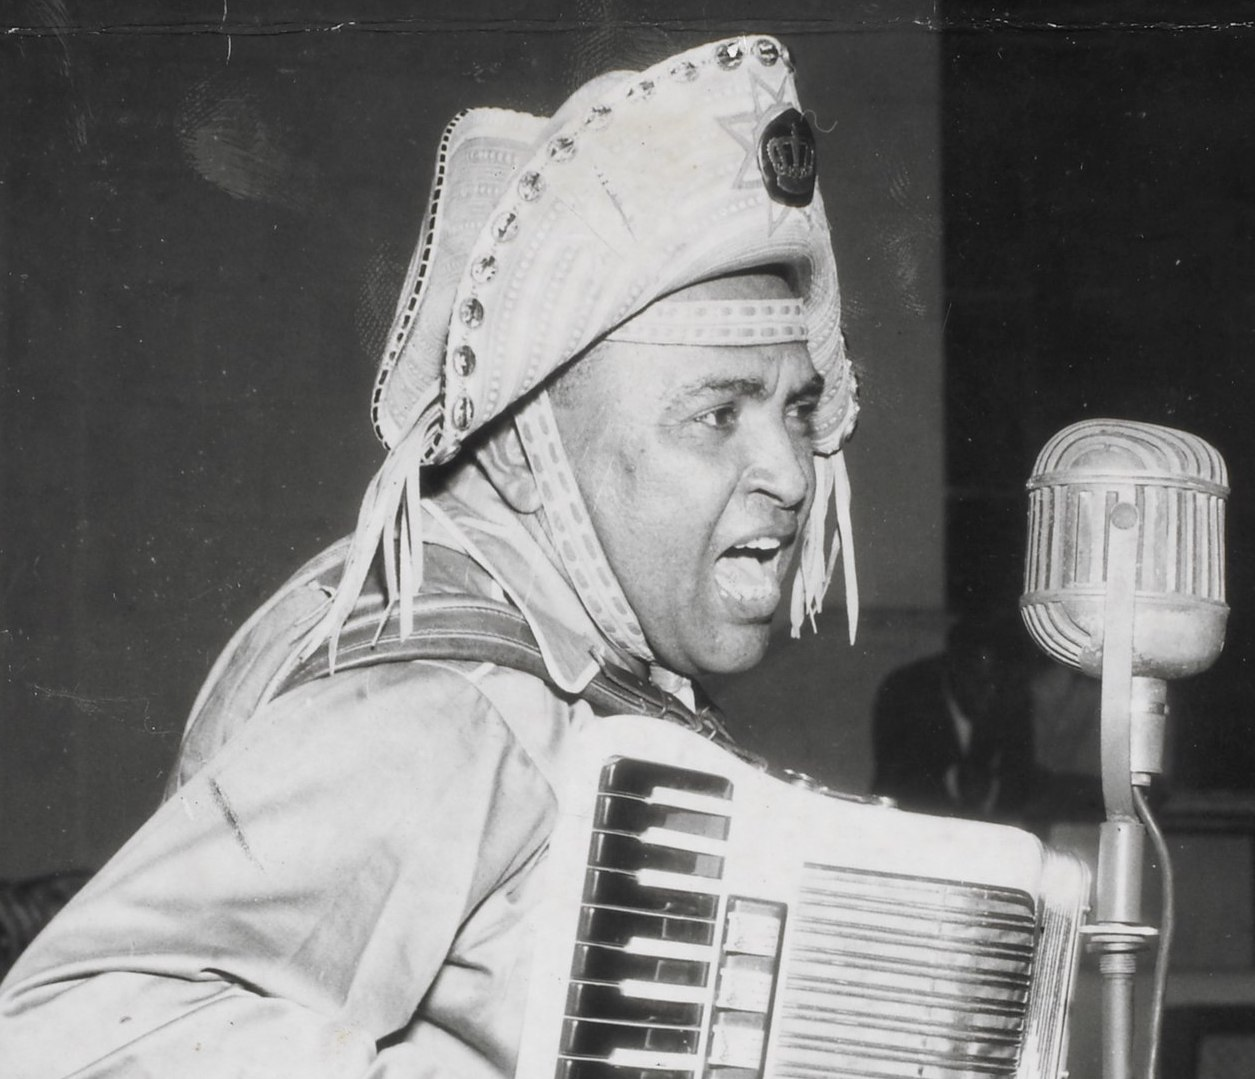
\includegraphics{fig3-gonzaga.jpg} \emph{Figure 1. Luiz Gonzaga, 1957.
From the Arquivo Nacional, public domain,
\href{https://en.wikipedia.org/wiki/Luiz_Gonzaga\#/media/File:Luiz_Gonzaga_(1957).tif}{Link}}

By the 1950s, due in large part to the works of these
singer-songwriters, themes of \emph{brasilidade} centered on notions of
Brazil as a diverse, mixed-race nation had become commonplace in the
Brazilian culture industry. For some, this was a welcome development.
Songs such as ``Asa Branca'' were celebrated for bringing the
experiences of Brazil's marginalized groups to national prominence in
new and powerful ways. Similarly, Caymmi's rich lyrical depictions of
Afro-Brazilian cultural life from the perspective of an insider ensured
that Black Brazilian narratives would not be left out of the national
cultural conversation. At the same time, many of the country's enduring
fault lines of inequality remained unaddressed, both in the cultural and
political realms. These themes would emerge as central issues in the
ensuing decades.

\section*{Part 2}

The mid-1950s saw the first of a series of seismic social and political
shifts that would transform Brazilian musical culture on a foundational
level. From 1956 to 1960, as part of national modernization efforts,
President Juscelino Kubitschek led a successful push to build a planned
city called Brasília to serve as Brazil's capital, moving the political
center from Rio de Janeiro. Then, in 1964, in response to progressive
economic reforms by democratically-elected left-wing President João
Goulart, the Brazilian military enacted a \emph{coup d'état} and
installed a military dictatorship that would last for twenty-one years.
Despite the restrictions of the military regime, the dictatorship saw
the emergence of a powerful network of Black activists, writers, and
artists that would become known as the Brazilian Black Consciousness
Movement. Across each of these moments, Brazilian popular song acted as
a key site for political activism and social commentary. The latter half
of the twentieth century also saw the emergence of new musical genres
from artists who were reconfiguring existing Brazilian musical practices
in new and transformative ways. This engagement with international
styles reflected the country's lasting dialogue with cultural producers
in the broader global sphere.

\hypertarget{bossa-nova}{%
\subsection*{Bossa Nova}\label{bossa-nova}}

In the late 1950s, the Brazilian popular music sphere was upended by the
emergence of bossa nova. Based in Rio de Janeiro and led by figures such
as composer Antonio Carlos ``Tom'' Jobim, lyricist Vinicius de Moraes,
and guitarist and vocalist João Gilberto, bossa nova reinvented the
profile of Brazilian popular song. Certain core elements of the genre
maintained stylistic elements from samba: Gilberto famously incorporated
characteristic \emph{tamborim} patterns from parading samba groups into
the iconic ``stuttering'' pattern of his guitar---a motif that is
apparent in the first recorded bossa nova song, ``Chega de Saudade''
(``No More Longing''; see Reily 1996, 4-5). Other elements departed in
more marked ways. Gilberto's soft, nasal vocal timbre represented a
sharp contrast with the belting style of Carnival and the rich delivery
common in \emph{samba-canção}.\footnote{Tatit ties these developments to
  a reaction against ``a certain stylistic excess'' present in
  \emph{samba-canção}, and likens bossa nova to a mode of
  ``re-establishing equilibrium'' in that regard (2002, 49).} Jobim
incorporated complex melodic and harmonic qualities that drew from
modernist composition and jazz---a combination that inspired Jobim,
Gilberto, and de Moraes's ironic song ``Desafinado'' (``Out of Tune'').
Bossa nova songs often digressed from the overtly nationalist lyrical
subject matter of previous eras, opting instead for low-key portraits of
upper-middle class life in Rio's cosmopolitan Zona Sul (South Zone).
These themes were perhaps best encapsulated in Jobim, de Moraes, and
Gilberto's ``Garôta de Ipanema'' (``The Girl from Ipanema''), performed
by Gilberto in collaboration with singer Astrud Gilberto and US
saxophonist Stan Getz, which painted a portrait of love and longing in
Rio's iconic Ipanema neighborhood. ``Garôta de Ipanema'' became the
basis for a worldwide explosion of the genre, which became
internationally popular in the early 1960s due in large part to
collaborations between musicians such as Gilberto and Getz.

\hypertarget{mpb-and-the-festival-era}{%
\subsection*{MPB and the Festival Era}\label{mpb-and-the-festival-era}}

The subdued cosmopolitanism of bossa nova gave way to a markedly
different tone in the wake of the 1964 Brazilian \emph{coup d'état}.
These events provoked a pronounced reaction among songwriters\emph{.}
Nowhere was this shift more pronounced than in the Festivals of Popular
Song, a series of contests hosted in São Paulo and Rio de Janeiro in
which the country's leading musicians wrote and performed songs that
were broadcast nationally. As part of an emergent reaction against
international styles of popular music such as rock `n' roll, songwriters
intentionally foregrounded genres native to Brazil, including samba,
bossa nova, and folkloric regional genres like \emph{baião}. Many of
their works have since become conceptualized under the broad generic
designation of MPB (Música Popular Brasileira, or Brazilian Popular
Music), an umbrella term that characterizes the stylistically diverse
popular songs that first emerged during the festival era (Moehn 2012,
17; Napolitano 1998; Reily 2000). Several songs became lasting national
favorites. Elis Regina's performance of ``Arrastão'' (``Trawler''), for
instance, in the 1965 Festival da Música Popular Brasileira, turned
Regina into a national icon for her powerful and arresting vocal
delivery that contrasted with the softer profile of bossa nova (Video
3). Others foregrounded implicit political messages. At the 1967 TV
Record Festival, Edu Lobo and Marília Medalha's \emph{baião-}inspired
``Ponteio'' (``Strumming''), declared, ``I won't leave behind my guitar
/ I'll see the times change / and a new place to sing,'' while Chico
Buarque's ``Roda Viva'' (``Wheel of Life'') proclaimed ``We want to have
an active voice / To lead in our destiny'' (Dunn 2001, 63-64).

\emph{Video 3. Elis Regina performing ``Arrastão'' during the 1965
Primeiro Festival de Música Popular Brasileira}

\hypertarget{tropicuxe1lia}{%
\subsection*{Tropicália}\label{tropicuxe1lia}}

The nationalist bent of the festival era was disrupted in 1967 with the
advent of Tropicália (alternately, Tropicalismo), a countercultural
project that critiqued Brazilian popular culture and rejected the
dictates of both the right- and left-wing (Dunn 2001; Napolitano 1998).
The figures associated with Tropicália included visual artists, poets,
and musicians, but the project found its most resonant and lasting
effects in the realm of popular song. Its storied debut took place in
the São Paulo-based 1967 TV Record festival, during which Gilberto Gil
and rock trio Os Mutantes (also from São Paulo) performed ``Domingo No
Parque'' (``Sunday In the Park''), which mixed capoeira and rock, and
Caetano Veloso performed ``Alegria, Alegria'' (``Joy, Joy''), which
fused Brazilian \emph{marcha} and rock (see Video 4). Over the next year
and a half, Gil and Veloso, along with an ensemble of musicians that
became known as the ``Bahian Group,'' released a series of landmark
songs (Figure 2). Some incorporated formal experimentation. Gil and
Veloso's song ``Batmacumba,'' for instance, drew lyrical inspiration
from the ideograms of Brazilian concrete poetry (Perrone 1985, 62).
Others introduced various forms of social commentary, such as Veloso and
Gal Costa's ironic critique of consumer culture in ``Baby'' or Veloso's
chaotic performance of ``É Proibido Proibir'' (``It is Forbidden to
Forbid'') at the 1968 Festival Internacional de Canção in defiance of
the event's prohibition of electric instruments. The Tropicálist project
came to an abrupt end in December 1968 with the Fifth Institutional Act
(AI-5), which cracked down on open speech and forced musicians such as
Gil and Veloso into exile.

\emph{Video 4. Gilberto Gil performing ``Domingo no Parque'' at the 1967
TV Record Festival}

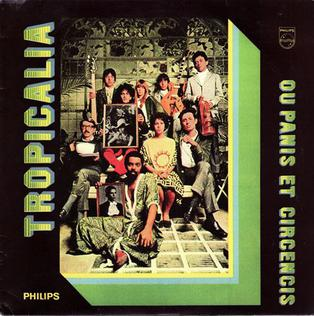
\includegraphics{fig5-tropicalia.jpg} \emph{Figure 2. The ``Bahian
Group'' on the cover of the 1968 album} Tropicália ou panis et
circencis. \emph{Clockwise from top right: Tom Zé, Torquato Neto, Gal
Costa, Gilberto Gil, Rogério Duprat, Arnaldo Baptista, Caetano Veloso,
Rita Lee, and Sérgio Dias, fair use,
\href{https://en.wikipedia.org/wiki/Tropicália:_ou_Panis_et_Circencis\#/media/File:Tropicália_LP.JPG}{Link}}

\hypertarget{black-soul-and-the-brazilian-black-consciousness-movement}{%
\subsection*{Black Soul and the Brazilian Black Consciousness
Movement}\label{black-soul-and-the-brazilian-black-consciousness-movement}}

Despite the military regime's restrictions on political speech, popular
song continued to serve as a vehicle for social expression in the wake
of AI-5. During this time, the Brazilian Black Consciousness Movement
emerged as a nationwide network of activists and initiatives that called
attention to endemic racism in Brazilian society and emphasized the
presence of a distinctly Black Brazilian identity.\footnote{Alberto
  2009, 19-20. As in many countries in Latin America, not all
  individuals of African heritage in Brazil have historically
  self-identified as Black. For this reason, when referring to all
  people of African descent, I follow the Brazilian norm and employ the
  term ``Afro-descendent,'' while reserving the term ``Black'' solely
  for those who self-identify as such.} Activist musicians sought in
particular to challenge the prevailing Brazilian ideology of racial
democracy, which denied the existence of racism in Brazil---a
challenging task given the frequent suppression of antiracist movements
by the military dictatorship, which viewed them as subversive. One
1970s-era musical iteration of this was the Rio de Janeiro-based
cultural movement known as Black Soul, in which artists such as Tim Maia
and groups such as Banda Black Rio and Abolição adapted US genres such
as soul and funk (Video 5 and Figure 3). This served as part of a
broader reaction against samba, which many Black musicians saw as
de-politicized and co-opted by white musicians. Many songs of the era
were explicitly political, such as Maia's ``Rodésia'' (``Rhodesia''),
which addressed decolonization in Africa. They formed part of a wider
phenomenon in which Black popular musicians celebrated the previously
marginalized figures of Black Brazilian political history. Jorge Ben's
1974 song ``Zumbi,'' for instance, along with his later funk-inspired
remake ``Zumbi (África Brasil),'' celebrated the seventeenth-century
anti-slavery \emph{quilombo} (maroon) leader Zumbi dos Palmares.

\emph{Video 5. Tim Maia performing ``Gostava Tanto de Você'' in 1989}

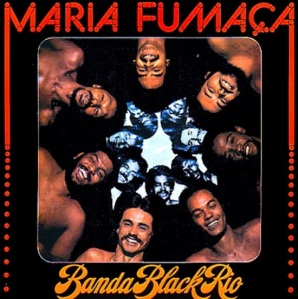
\includegraphics{fig6-maria-fumaca.jpg} \emph{Figure 3. The cover of
Banda Black Rio's 1977 album} Maria Fumaça, \emph{fair use,
\href{https://en.wikipedia.org/wiki/Maria_Fumaça\#/media/File:Bandablackrio-mariafumaca1977.jpg}{Link}}

\hypertarget{popular-song-and-the-northeastern-black-brazilian-carnival}{%
\subsection*{Popular Song and the Northeastern Black Brazilian
Carnival}\label{popular-song-and-the-northeastern-black-brazilian-carnival}}

In the Brazilian Northeast, Black popular song often drew from
Afro-Brazilian Carnival practices circulating in the region. Perhaps the
most iconic instance of this phenomenon came from the \emph{blocos
afros} movement, in which African-themed parading Carnival groups
promoted a ``re-Africanized'' form of samba and openly confronted racism
(Risério 1981). Gilberto Gil's 1977 album \emph{Refavela}, for instance,
featured a cover of the song ``Que Bloco É Esse'' (``What \emph{Bloco}
Is That?''), written by the first \emph{bloco afro,} Ilê Aiyê (Video 6).

\emph{Video 6. Ilê Aiyê in the 2016 Carnival in Salvador da Bahia}

In 1986, the \emph{bloco afro} Olodum pioneered the genre of
\emph{samba-reggae} with the nationally popular hit Carnival song
``Faraó, Divinidade do Égito'' (``Pharaoh, Divinity of Egypt,'' Video
7). The national popularity of \emph{samba-reggae} inspired the Bahian
genre of \emph{axé}, which integrated the sounds of the Bahian Carnival
and other popular styles with lyrics that celebrated Afro-Brazilian
cultural practices and heritage. \emph{Axé} songs such as Margareth
Menezes's ``Faraó'' (a cover of Olodum's hit) and Daniela Mercury's
``Swing da Cor'' (``Swing of Color'') helped to foreground the cultural
landscape of Bahia in the Brazilian culture industry to an unprecedented
degree, including its racial politics.

\emph{Video 7. Olodum performing} samba-reggae \emph{in Salvador da
Bahia, 2011}

These figures formed part of a broader spectrum of groups that drew from
the distinct Carnival practices of the Brazilian Northeast, including
other regional Carnival genres from Pernambuco such as \emph{frevo} and
\emph{maracatu}. Perhaps most iconically, the Recife-based group Chico
Science and Nação Zumbi led the 1990s-era musical movement of
\emph{manguebeat}, which situated critiques of local social issues
within music that drew from \emph{maracatu} along with rock, funk, and
hip hop, as in the songs ``Rios, Pontes, e Overdrives'' (``Rivers,
Bridges, and Overdrives'') and ``Maracatu Atômico'' (``Atomic
Maracatu,'' Video 8).

\emph{Video 8. Music video of Chico Science and Nação Zumbi's song
``Maracatu Atômico''}

\hypertarget{experimentations}{%
\subsection*{Experimentations}\label{experimentations}}

Popular song has long offered a site for more radical forms of invention
as well. In the wake of AI-5, the 1970s saw an unprecedented period of
formal experimentation by popular songwriters such as Veloso, Tom Zé,
and Walter Franco. Veloso's \emph{Araça Azul} (1972), for instance,
famously became the most returned album in the history of Brazilian
popular music due to its rejection of the structural elements of popular
song in favor of experimental textures such as collage and
unintelligible lyrics. In \emph{Estudando o Samba} (1976), Zé
incorporated ironic lyrical narratives within stripped-down
pastiche-like takes on samba and non-lyrical material such as samples of
screams and recorded noise. In the late 1970s and early 80s, São Paulo
became a hub for departures from the conventional profile of popular
song with a series of productions by artists affiliated with the
independent publishing house and concert venue Lira Paulistana. Arrigo
Barnabé, in his album \emph{Clara Crocodilo} (1980), famously wrote
songs that integrated rock and jazz with 12-tone composition, while
Itamar Assumpção's LP \emph{Beleleu, Leleu, Eu} (1980) mixed
straightforward fare with elements of collage and pastiche. Throughout
these moments, Zé remained a central figure. His 1998 album \emph{Com
Defeito de Fabricação} (\emph{Fabrication Defect}), for instance,
introduced the notion of the ``aesthetics of plagiarism,'' in which each
song on the album appropriated external artistic material and
recontextualized them into a new ``plagiarized'' context.\footnote{Zé's
  songs on \emph{Com Defeito de Fabricação} incorporated a wide and
  eclectic range of sources, from 1950s-era concrete poetry (in the
  track ``O Olho do Lago'') to Rimsky Korsakov (in the track
  ``Politicar''). J. Griffith Rollefson has characterized this as a
  model for strategic appropriation of First World material by oppressed
  Third World subjects in order to articulate a new, empowered hybrid
  subjectivity in today's postmodern and postcolonial era (Rollefson
  2007, 310). Zé characterized each of the songs in \emph{Com Defeito de
  Fabricação} as different kind of \emph{arrastão} (dragnet) of external
  artistic material, and argued that this heralded the end of the
  ``composer's era'' and inaugurated the ``plagi-combinator era.''}

\hypertarget{contemporary-popular-song}{%
\subsection*{Contemporary Popular Song}\label{contemporary-popular-song}}

Popular song remains a pillar of the Brazilian culture industry.
Song-based genres such as \emph{sertanejo}, \emph{axé}, and
\emph{pagode} dominate the proverbial airwaves, along with songs drawing
from internationally circulating popular genres. In the political arena,
songs such as Caetano Veloso and Daniela Mercury's ``Proibido o
Carnaval'' (``Forbidden Carnival,'' Video 9) and Luedji Luna's ``Um
Corpo no Mundo'' (``A Body in the World'') offer a site for confronting
the country's reactionary turn under Jair Bolsonaro, who has celebrated
authoritarianism and disparaged the country's nonwhite and LGBTQ+
populations.

\emph{Video 9. Music video of Daniela Mercury and Caetano Veloso's 2019
song ``Proibido o Carnaval''}

Building on the Brazilian Black Consciousness Movement's legacy of
activism, many songwriters have tapped into antiracist themes
circulating in the international sphere---a phenomenon that was embodied
in 2020 when Gabriel Moura collaborated with Banda Black Rio to produce
the song ``Vidas Negras Sim Importam'' (``Black Lives Do Matter''). The
landscape in which contemporary popular musicians operate also affords
space for departures from the form. The trio Metá Metá's album
\emph{MM3}, for instance, integrates genres such as samba and rock with
free jazz-inflected improvisations and traditional material from the
Afro-Brazilian religion of Candomblé, while Cadu Tenório and Márcio
Bulk's LP \emph{Banquete} situates songs in the style of midcentury
\emph{samba-canção} within harsher textures drawing from industrial rock
and harsh noise.

Today, Brazilian popular song continues as a form in flux, grounded in a
rich yet complex history of lyrical and melodic expressivity,
experimentation, and social engagement. Despite the profound shifts
Brazilian society has undergone over the past century, the issues that
shaped popular song since the beginning of the twentieth century remain
front-and-center. Racial and socioeconomic inequality continues to
impede social progress. Differing ideas about Brazilian national
identity remain hotly contested. And with the rise of neo-authoritarian
politics, the country's political circumstances are the most uncertain
they have been since the fall of the dictatorship. As these concerns are
negotiated, one outcome seems certain: popular song will persist at the
center of Brazilian cultural discourse, whether in negotiating
disagreement, expressing resistance, or capturing moments of shared joy.



\hypertarget{discussion-questions}{%
\section*{Discussion Questions}\label{discussion-questions}}

\begin{enumerate}
\def\labelenumi{\arabic{enumi}.}
\item
  How has music been used as a vehicle for antiracist activism in
  Brazil? What parallels do you see between antiracist popular songs in
  Brazil and similar movements in the international sphere?
\item
  What kind of image of the nation of Brazil did nationalist popular
  songs seek to create? How has this changed over time? Is this image
  similar to how you think about your country?
\item
  Brazilian songwriters have often faced suppression and censorship from
  authoritarian government figures. How have Brazilian popular
  songwriters enacted social critiques in their songs despite these
  restrictions?
\item
  What are some of the ways that Brazilian popular song was influenced
  by international genres of popular music? What are some of the ways in
  which Brazilian popular song sounded back out into the international
  sphere in turn?
\item
  Watch a video of \emph{maracatu} in the Recife Carnival, then watch
  the music video of Chico Science and Nação Zumbi's song ``Maracatu
  Atômico.'' Can you see or hear any similarities? How are the videos
  different?
\item
  Compare the music of the Bahian Carnival to its adaptations in the
  popular sphere. First, listen to Ilê Aiyê's 1975 song ``Que Bloco É
  Esse?'' (an example of \emph{samba-afro}) and Gilberto Gil's 1977
  cover of that same song, ``Ilê Aiyê.'' Then, listen to Olodum's 1986
  song ``Faraó, Divinidade do Égito'' (an example of
  \emph{samba-reggae}) and Margareth Menezes's 2004 cover of that same
  song, ``Faraó.'' How did the songs change as they were adapted into
  the popular sphere via the recording industry?
\item
  Listen to ``Chega de Saudade'' and ``Garôta de Ipanema,'' then listen
  to Eydie Gormé's ``Blame it on the Bossa Nova'' and Elvis Presley's
  ``Bossa Nova Baby,'' both of which were written during the period in
  which bossa nova became globally popular. If you were a bossa nova
  musician, what would you think of these adaptations?
\item
  Watch a video of Elis Regina's ``Arrastão,'' Chico Buarque's ``Roda
  Viva,'' Gilberto Gil's ``Domingo no Parque,'' or Caetano Veloso's
  ``Alegria, Alegria,'' all of which took place during the era of the
  1960s Festivals of Popular Song. Describe the scene: the energy of the
  space, the theatricality of the performances, the sonic qualities of
  the performance, the interactions between musicians and audience. What
  do these qualities say about the place of popular song in Brazilian
  culture during this time period?
\end{enumerate}

\hypertarget{works-cited}{%
\section*{Works Cited}\label{works-cited}}

\{:.hang\} Alberto, Paulina. 2009. ``When Rio Was Black: Soul Music,
National Culture, and the Politics of Racial Comparison in 1970s
Brazil.'' \emph{The Hispanic American Historical Review} 89, no. 1:
3-39.

\{:.hang\} Araújo, Hiram\emph{.} 2012. \emph{A Cartilha das Escolas de
Samba}. Rio de Janeiro: Centro de Memória do Carnaval LIESA.

\{:.hang\} Arinos, Afonso. 1917. \emph{A unidade da Pátria: conferência
que fez o Dr.~Affonso Arinos, no festival realisado em Bello Horizonte,
em benefício dos flagellados.} Rio de Janeiro: Livr. F. Alves.

\{:.hang\} Dunn, Christopher. 2001. \emph{Brutality Garden: Tropicália
and the Emergence of a Brazilian Counterculture.} Chapel Hill: UNC Press
Books.

\{:.hang\} Hertzman, Marc. 2013. \emph{Making Samba: A New History of
Race and Music in Brazil.} Durham, NC: Duke University Press.

\{:.hang\} Loveless, Megwen. 2012. ``Between the Folds of Luiz Gonzaga's
Sanfona: \emph{Forró} Music in Brazil,'' in \emph{The Accordion in the
Americas: Klezmer, Polka, Tango, Zydeco, and More!}, edited by Helena
Simonett, 268-294. Urbana: University of Illinois Press.

\{:.hang\} McNally, James. 2021. ``The End of Song: Improvisation as
Social Critique in Brazil.'' \emph{Twentieth-Century Music} 18, no. 1:
125-152.

\{:.hang\} Moehn, Frederick. 2012. \emph{Contemporary Carioca:
Technologies of Mixing in a Brazilian Music Scene.} Durham, NC: Duke
University Press.

\{:.hang\} Napolitano, Marcos. 1998. ``A Invenção da Música Popular
Brasileira: Um Campo de reflexão para a História Social,'' \emph{Latin
American Music Review} 19, no. 1: 92-105.

\{:.hang\} ­­­------. 2001. \emph{Seguindo a canção: engajamento
politico e indústria cultural na MPB, 1959-69.} São Paulo: Annablume.

\{:.hang\} Perrone, Charles. 1985. ``From Noigandres to `Milagre da
Alegria:' The Concrete Poets and Contemporary Brazilian Popular Music.''
\emph{Latin American Music Review} 6, no. 1: 58-79.

\{:.hang\} Raymundo, Jackson. 2019. ``O samba-enredo e a formação de uma
Poética da Brasilidade.'' \emph{SEDA-Revista de Letras da Rural-RJ} 4,
no. 10: 120-137.

\{:.hang\} Reily, Suzel Ana. 2000. ``Introduction: Brazilian Musics,
Brazilian Identities.'' \emph{Ethnomusicology Forum} 9, no. 1: 1-10.

\{:.hang\} Risério, António. 1981. \emph{Carnaval Ijexá.} Salvador:
Corrupio.

\{:.hang\} Rollefson, J. Griffith. 2007. ``Tom Ze's Fabrication Defect
and the `Esthetics of Plagiarism': A Postmodern/Postcolonial
`Cannibalist Manifesto.'\,'' \emph{Popular Music and Society} 30, no. 3:
305--27.

\{:.hang\} Tatit, Luiz. 1996. \emph{O cancionista}. São Paulo: Edusp.

\{:.hang\} ­­­------. 2004. \emph{O século da canção.} São Paulo: Ateliê
Editorial.

\{:.hang\} ­­­------. 2002. `Analysing Popular Songs.' In \emph{Popular
Music Studies}, trans. Lorraine Leu, edited by David Hesmondhalgh and
Keith Negus, 33-50. London: Arnold.

\{:.hang\} Vianna, Hermano. 1999. \emph{The Mystery of Samba: Popular
Music \& National Identity in Brazil}, edited and translated by John
Charles Chasteen. Chapel Hill: The University of North Carolina Press.


\end{document}